\documentclass{article}
\usepackage{amsmath,listings,tikz, float}
\title{genesis}
\author{Eric Caleb}
\date{\today}

\begin{document}
  \maketitle
  Below are some solutions of equations and code.

  \section{Equations}

    \begin{equation}
        a^2 + b^2 = c^2
    \end{equation}

    \begin{figure}[H]
        \centering
            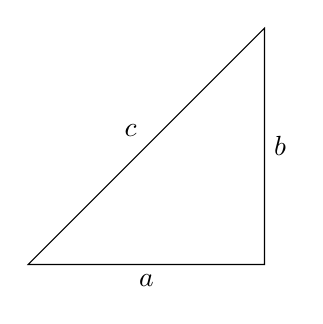
\begin{tikzpicture}
                % \draw (0,0) -- (1,1) -- (1,0) -- cycle;
                \draw (0,0) -- (3,3) node[midway, above left] {$c$}
                              -- (3,0) node[midway, right] {$b$}
                              -- cycle node[midway, below] {$a$};
            \end{tikzpicture}
            \caption{A simple triangle}
    \end{figure}


  \section{Code}

    \begin{lstlisting}
        import numpy as np
        import matplotlib.pyplot as plt

        x = np.linspace(0, 10, 100)
        y = np.sin(x)
        plt.plot(x, y)
        plt.show()

    \end{lstlisting}
  \end{document}
